\documentclass[aspectratio=169]{beamer}

% Compile from this directory:  pdflatex slides.tex  (run twice)

% Theme selection
\usetheme{Madrid}
\usecolortheme{whale}
\usefonttheme[onlymath]{serif}

% Packages
\usepackage{graphicx}
\usepackage{booktabs}
\usepackage{tikz}
\usetikzlibrary{shapes, positioning, shadows, arrows.meta, fit, backgrounds, calc}
\usepackage{amsmath}
\usepackage{amssymb}
\usepackage{hyperref}
\usepackage{listings}
\usepackage{multirow}
\usepackage{colortbl}

\graphicspath{{figures/}}

% Warm academic-gold palette
\definecolor{deepgold}{RGB}{112, 78, 0}
\definecolor{medgreen}{RGB}{91, 116, 48}
\definecolor{alertred}{RGB}{166, 70, 32}
\definecolor{darkred}{RGB}{130, 45, 24}
\definecolor{amber}{RGB}{214, 145, 0}
\definecolor{violet}{RGB}{126, 92, 112}
\definecolor{papercream}{RGB}{255, 252, 237}
\definecolor{goldenbar}{RGB}{151, 103, 0}
\definecolor{sunlight}{RGB}{247, 211, 103}
\definecolor{warmink}{RGB}{62, 47, 14}

% Theme application
\setbeamercolor{normal text}{fg=warmink, bg=papercream}
\setbeamercolor{background canvas}{bg=papercream}
\setbeamercolor{structure}{fg=goldenbar}
\setbeamercolor{frametitle}{bg=goldenbar, fg=white}
\setbeamercolor{titlelike}{bg=goldenbar, fg=white}
\setbeamercolor{palette primary}{bg=goldenbar, fg=white}
\setbeamercolor{palette secondary}{bg=amber, fg=warmink}
\setbeamercolor{palette tertiary}{bg=deepgold, fg=white}
\setbeamercolor{palette quaternary}{bg=sunlight, fg=warmink}
\setbeamercolor{block title}{bg=goldenbar, fg=white}
\setbeamercolor{block body}{bg=sunlight!18, fg=warmink}
\setbeamercolor{block title alerted}{bg=alertred, fg=white}
\setbeamercolor{block body alerted}{bg=alertred!9, fg=warmink}
\setbeamercolor{block title example}{bg=medgreen, fg=white}
\setbeamercolor{block body example}{bg=medgreen!10, fg=warmink}
\setbeamercolor{item projected}{bg=goldenbar, fg=white}
\setbeamercolor{section in toc}{fg=deepgold}

\setbeamertemplate{navigation symbols}{}
\setbeamerfont{caption}{size=\scriptsize}

% Title Info
\title[IPL Lab]{VTool-R1: VLMs Learn to Think with Images via Reinforcement Learning on Multimodal Tool Use}
\subtitle{Paper by M.~Wu, J.~Yang, J.~Jiang, M.~Li, K.~Yan, H.~Yu, M.~Zhang, C.~Zhai, K.~Nahrstedt\\
  (UIUC \& U.~Michigan) \quad arXiv:2505.19255}
\author[Shayan Salehi]{Shayan Salehi}
\institute[SUT]{
  Department of Computer Engineering\\
  Sharif University of Technology\\
  IPL Lab
}
\date{October 2026}

\begin{document}

% =============================================================================
\begin{frame}
  \titlepage
\end{frame}

\begin{frame}{Outline}
  \tableofcontents
\end{frame}

% =============================================================================
\section{Introduction \& Problem Statement}

\begin{frame}{Why Do VLMs Still ``Think'' Only in Text?}
  \begin{columns}[T]
    \column{0.55\textwidth}
    \small
    \textbf{Background:}
    \begin{itemize}
      \item RL fine-tuning (RFT) gave LLMs long CoT, self-correction and \textbf{learned tool use} (Search-R1).
      \item Recent VLM ``R1'' works (R1-V, Vision-R1, R1-VL, \dots) copy this recipe.
      \item \textcolor{alertred}{\textbf{But their reasoning stays text-driven:}} the image is
            encoded once; every later step is text.
    \end{itemize}
    \vspace{0.1cm}
    \textbf{Why it matters}
    \begin{itemize}
      \item A \emph{six-fingered} hand: ``how many fingers?'' $\rightarrow$ the text prior ``five'' can beat the pixels.
      \item Inference-time visual CoT (Visual Sketchpad, ReFocus) helps, but
            \textcolor{alertred}{only with GPT-4o-class models}; small open models fail.
    \end{itemize}
    \column{0.42\textwidth}
    \begin{block}{The Core Question}
      \small Can we \textbf{train} a small open VLM, with RL and only an outcome reward,
      to produce \emph{intermediate visual steps} (edited images) and reason over them,
      i.e.\ to ``think with images''?
    \end{block}
    \vspace{0.2cm}
    \begin{alertblock}{The Missing Piece}
      \small No prior RFT framework puts image-editing tool calls \emph{inside} the rollout,
      so the model never learns \emph{when} or \emph{how} to look again.
    \end{alertblock}
  \end{columns}
\end{frame}

\begin{frame}{Three Roadblocks to Multimodal Chains of Thought}
  \begin{enumerate}
    \setlength{\itemsep}{0.55cm}
    \item \textbf{\textcolor{deepgold}{Language shortcuts}}\\
      Text-only CoT lets the decoder drift to a plausible-sounding answer that the image
      contradicts; nothing forces the model to re-inspect visual evidence.
    \item \textbf{\textcolor{deepgold}{Prompting does not transfer to small models}}\\
      Prompted tool use works for GPT-4o, but open Qwen2.5-VL 3B/7B fail to follow
      tool-use instructions: prompting them to use tools \emph{lowers} accuracy (3B chart: 51.8 $\rightarrow$ 24.6).
    \item \textbf{\textcolor{deepgold}{Training with tools in the loop is awkward}}\\
      Generation must pause for external Python execution, the edited image must be fed
      back as a new input, and rewards on the tool calls themselves invite reward hacking.
  \end{enumerate}
\end{frame}

\begin{frame}{Proposed Solution: VTool-R1}
  \begin{columns}[T]
    \column{0.5\textwidth}
    \textbf{\textcolor{medgreen}{Contribution 1: RFT Framework with Visual Tools}}
    \begin{itemize}
      \item Python image-editing tools are executed \emph{during} RL rollouts.
      \item Two-pass rollout: reason $\rightarrow$ edit image $\rightarrow$ reason over
            original $\oplus$ edited image.
      \item Built on GRPO; trained with an \textbf{outcome-only} 0/1 reward.
    \end{itemize}
    \column{0.5\textwidth}
    \textbf{\textcolor{medgreen}{Contribution 2: First Learned ``Thinking with Images''}}
    \begin{itemize}
      \item Claimed first work to make VLMs \emph{learn} to interleave visual steps with text CoT.
      \item Model decides \emph{whether} a tool helps; it is never rewarded for using one.
      \item Validated on chart and table QA (ReFocus splits), Qwen2.5-VL 3B/7B/32B.
    \end{itemize}
  \end{columns}
  \vspace{0.6cm}
  \begin{center}
    \textbf{Goal:} turn ``visual editing as chain of thought'' from a GPT-4o-only prompting trick
    into a skill that small open VLMs acquire through RL.
  \end{center}
\end{frame}

\begin{frame}{Thinking with Images: What a Trained Rollout Looks Like}
  \centering
  \begin{figure}
    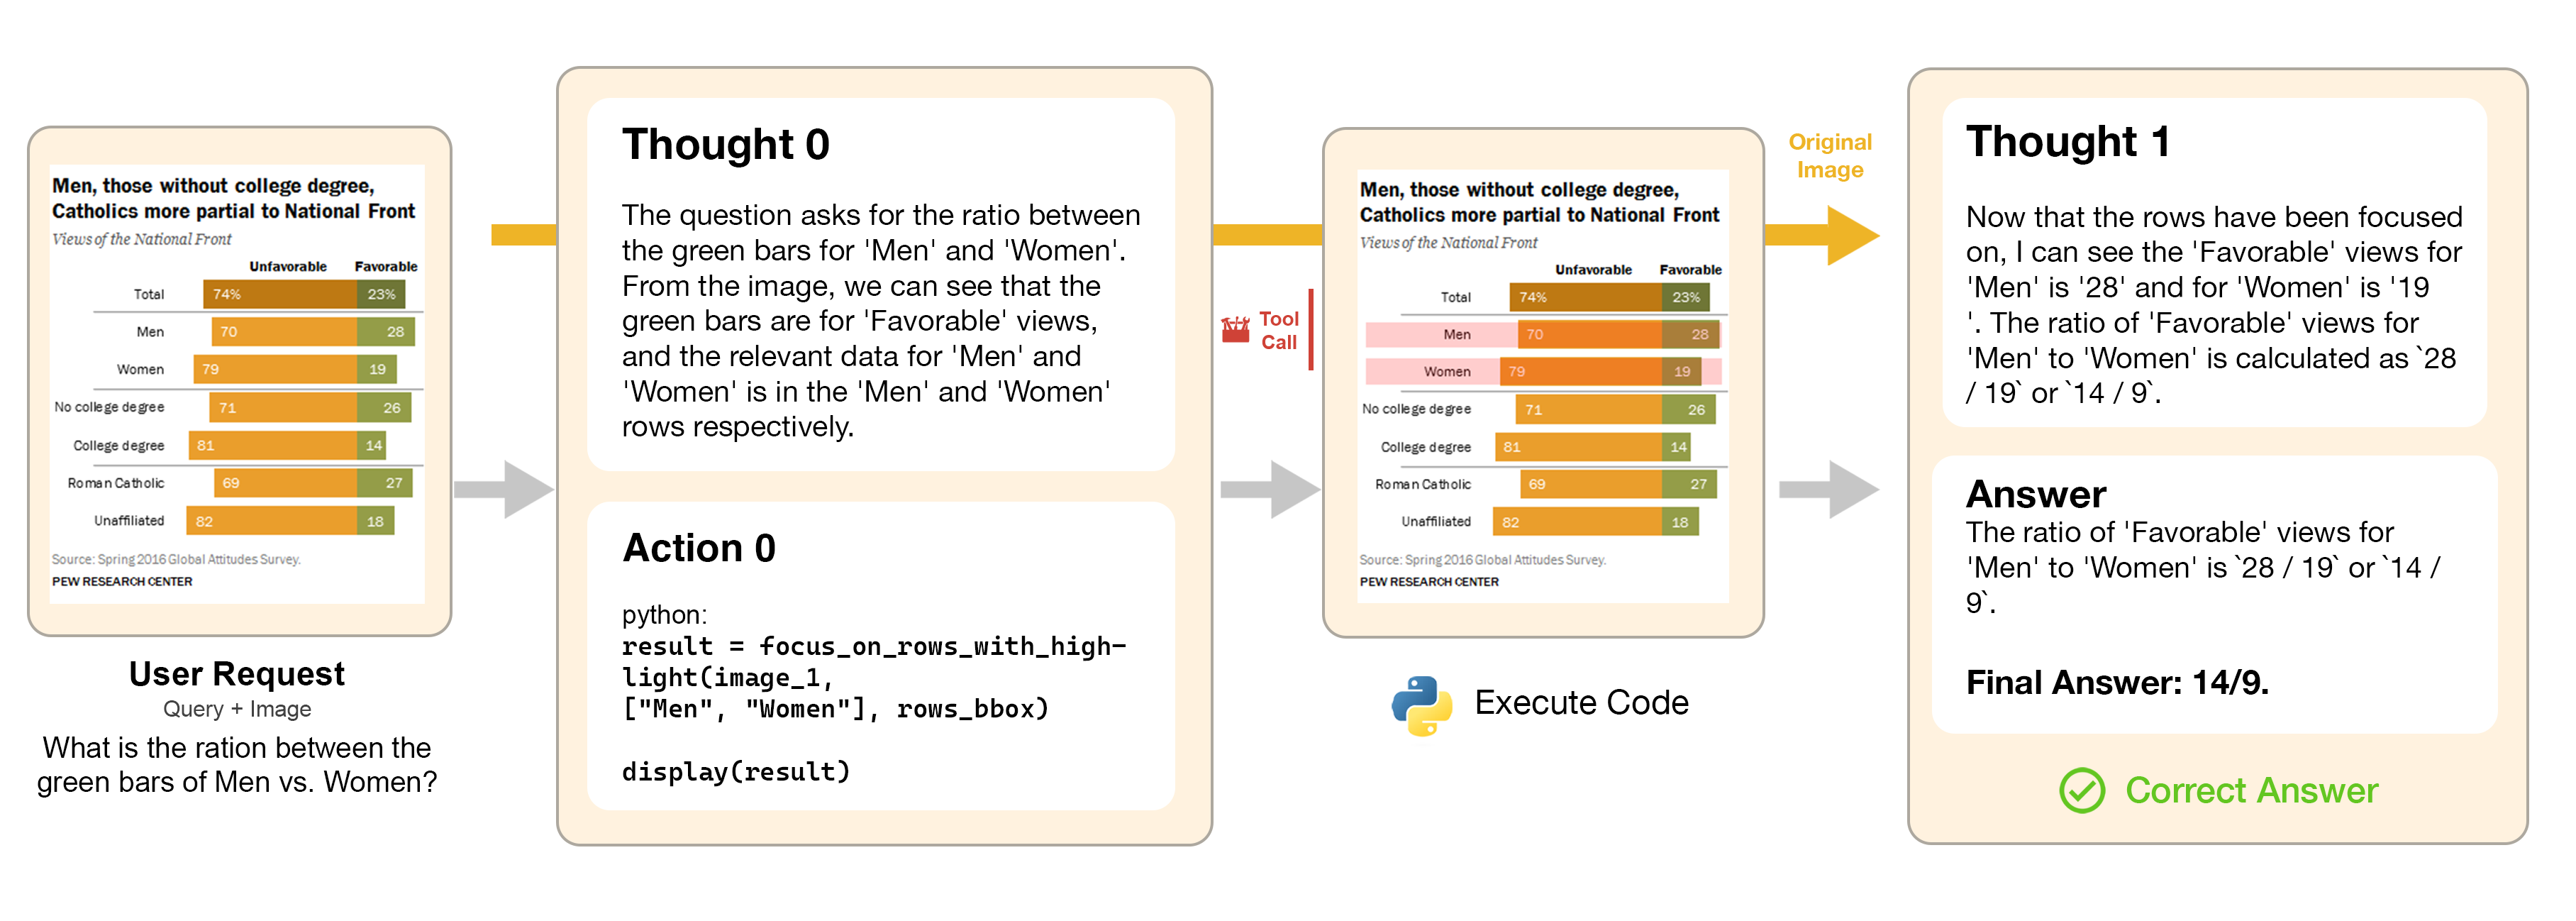
\includegraphics[width=0.97\textwidth]{vtool_example.png}
    \caption{After RFT, the 3B model reasons in \emph{Thought 0}, emits a tool call that highlights the
      ``Men'' and ``Women'' rows, receives the edited chart \emph{alongside} the original, and reads the
      ``Favorable'' values (28 vs.\ 19) in \emph{Thought 1}. The visual step narrows attention to
      exactly the evidence the question needs.}
  \end{figure}
\end{frame}

% =============================================================================
\section{Methodology}

\begin{frame}{Inference \& Rollout with a Visual Chain of Thought}
  \centering
  \resizebox{0.95\textwidth}{!}{%
  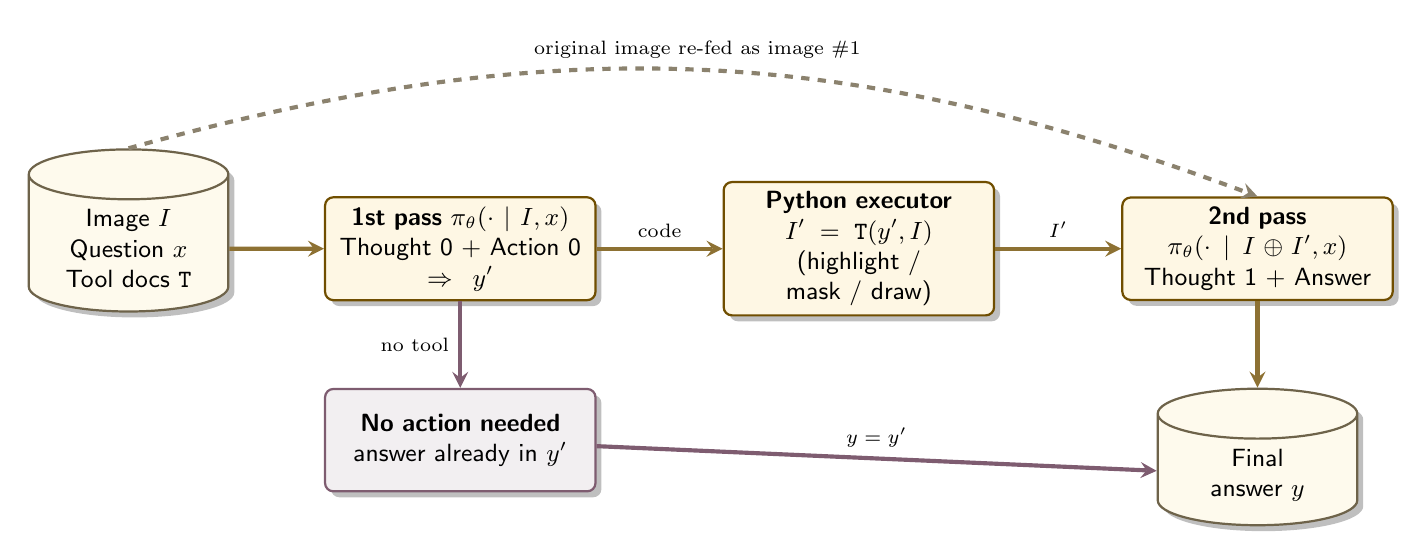
\begin{tikzpicture}[
      node distance=0.8cm and 1.2cm,
      font=\small\sffamily,
      >=stealth,
      block/.style={rectangle, rounded corners=3pt, draw=deepgold, thick,
                    fill=sunlight!18, text width=3.2cm, align=center,
                    minimum height=1.3cm, drop shadow},
      data/.style={cylinder, draw=warmink!75, thick, fill=sunlight!12,
                   shape border rotate=90, aspect=0.25, text width=2.3cm,
                   align=center, minimum height=1.3cm, drop shadow},
      arrow/.style={->, line width=1.5pt, draw=deepgold!80}
  ]
  \node[data] (input) {Image $I$\\Question $x$\\Tool docs \texttt{T}};
  \node[block, right=of input] (r1) {\textbf{1st pass} $\pi_\theta(\cdot\mid I,x)$\\Thought 0 + Action 0\\$\Rightarrow y'$};
  \node[block, right=1.6cm of r1] (exec) {\textbf{Python executor}\\$I' = \texttt{T}(y', I)$\\(highlight / mask / draw)};
  \node[block, right=1.6cm of exec] (r2) {\textbf{2nd pass} $\pi_\theta(\cdot\mid I\oplus I',x)$\\Thought 1 + Answer};
  \node[data, below=1.1cm of r2] (out) {Final\\answer $y$};
  \node[block, below=1.1cm of r1, fill=violet!10, draw=violet] (direct) {\textbf{No action needed}\\answer already in $y'$};

  \draw[arrow] (input) -- (r1);
  \draw[arrow] (r1) -- node[above, font=\scriptsize] {code} (exec);
  \draw[arrow] (exec) -- node[above, font=\scriptsize] {$I'$} (r2);
  \draw[arrow] (r2) -- (out);
  \draw[arrow, draw=violet] (r1) -- node[left, font=\scriptsize] {no tool} (direct);
  \draw[arrow, draw=violet] (direct) -- node[above, font=\scriptsize] {$y = y'$} (out);
  \draw[arrow, dashed, draw=warmink!60] (input.north) to[bend left=18]
        node[above, font=\scriptsize] {original image re-fed as image \#1} (r2.north);
  \end{tikzpicture}
  }
  \vspace{0.15cm}
  \begin{columns}[T]
    \column{0.5\textwidth}
    \small
    $$ y' \sim \pi_\theta(\cdot \mid I, x), \qquad I' = \texttt{T}(y', I) $$
    $$ y \sim \pi_\theta(\cdot \mid I, x; \texttt{T}) = \pi_\theta\big(\cdot \mid I \oplus \texttt{T}(y', I),\, x\big) $$
    \column{0.47\textwidth}
    \footnotesize
    \begin{itemize}
      \item $\oplus$: original and edited image given as \textbf{two image inputs} (needs a multi-image VLM).
      \item At most \textbf{one} tool turn; several tool calls may be chained inside it.
    \end{itemize}
  \end{columns}
\end{frame}

\begin{frame}{Prompt Format and the Visual Editing Toolset \texttt{T}}
  \begin{columns}[T]
    \column{0.47\textwidth}
    \textbf{\textcolor{deepgold}{Structured output format}}
    \vspace{0.1cm}

    \fcolorbox{deepgold}{white}{
      \parbox{0.92\textwidth}{\scriptsize\ttfamily
        \textcolor{goldenbar}{THOUGHT 0:} rows ``Men'' and ``Women'' hold the answer\\
        \textcolor{goldenbar}{ACTION 0:}\\
        \hspace*{1em}r = focus\_on\_rows\_with\_highlight(\\
        \hspace*{3em}image\_1, ["Men","Women"], rows\_bbox)\\
        \hspace*{1em}display(r)\\
        \textcolor{goldenbar}{OBSERVATION:} <edited image = image \#2>\\
        \textcolor{goldenbar}{THOUGHT 1:} Men = 28, Women = 19\dots\\
        \textcolor{goldenbar}{ANSWER:} \dots\ \textcolor{goldenbar}{FINAL ANSWER:} 14/9\\
        \textcolor{goldenbar}{TERMINATE}
      }
    }
    \vspace{0.2cm}

    \footnotesize
    Prompt includes tool signatures, 9 requirements (e.g.\ ``only one ACTION''),
    few-shot examples, and the \textbf{bounding boxes} of rows/columns (or chart bars).
    \column{0.5\textwidth}
    \textbf{\textcolor{deepgold}{Tools (Python + OpenCV, from ReFocus)}}
    \vspace{0.1cm}

    \renewcommand{\arraystretch}{1.25}
    \resizebox{\textwidth}{!}{%
    \begin{tabular}{lll}
      \toprule
      \textbf{Tool} & \textbf{Applies to} & \textbf{Effect} \\
      \midrule
      Highlight & columns / rows & semi-transparent red overlay \\
      Mask      & columns / rows & white mask over irrelevant parts \\
      Draw      & columns / rows & solid red bounding box \\
      \midrule
      Chart variants & bars (by $x$/$y$ value) & highlight / mask bars \\
      \bottomrule
    \end{tabular}}
    \vspace{0.3cm}

    \begin{block}{Intuition}
      \small Tools simulate \textbf{selective visual attention}: the model edits the image to
      isolate the evidence, then reads it again, as a human would with a highlighter.
    \end{block}
  \end{columns}
\end{frame}

\begin{frame}{Multi-Modal GRPO with Tool Use: Training Pipeline}
  \centering
  \begin{figure}
    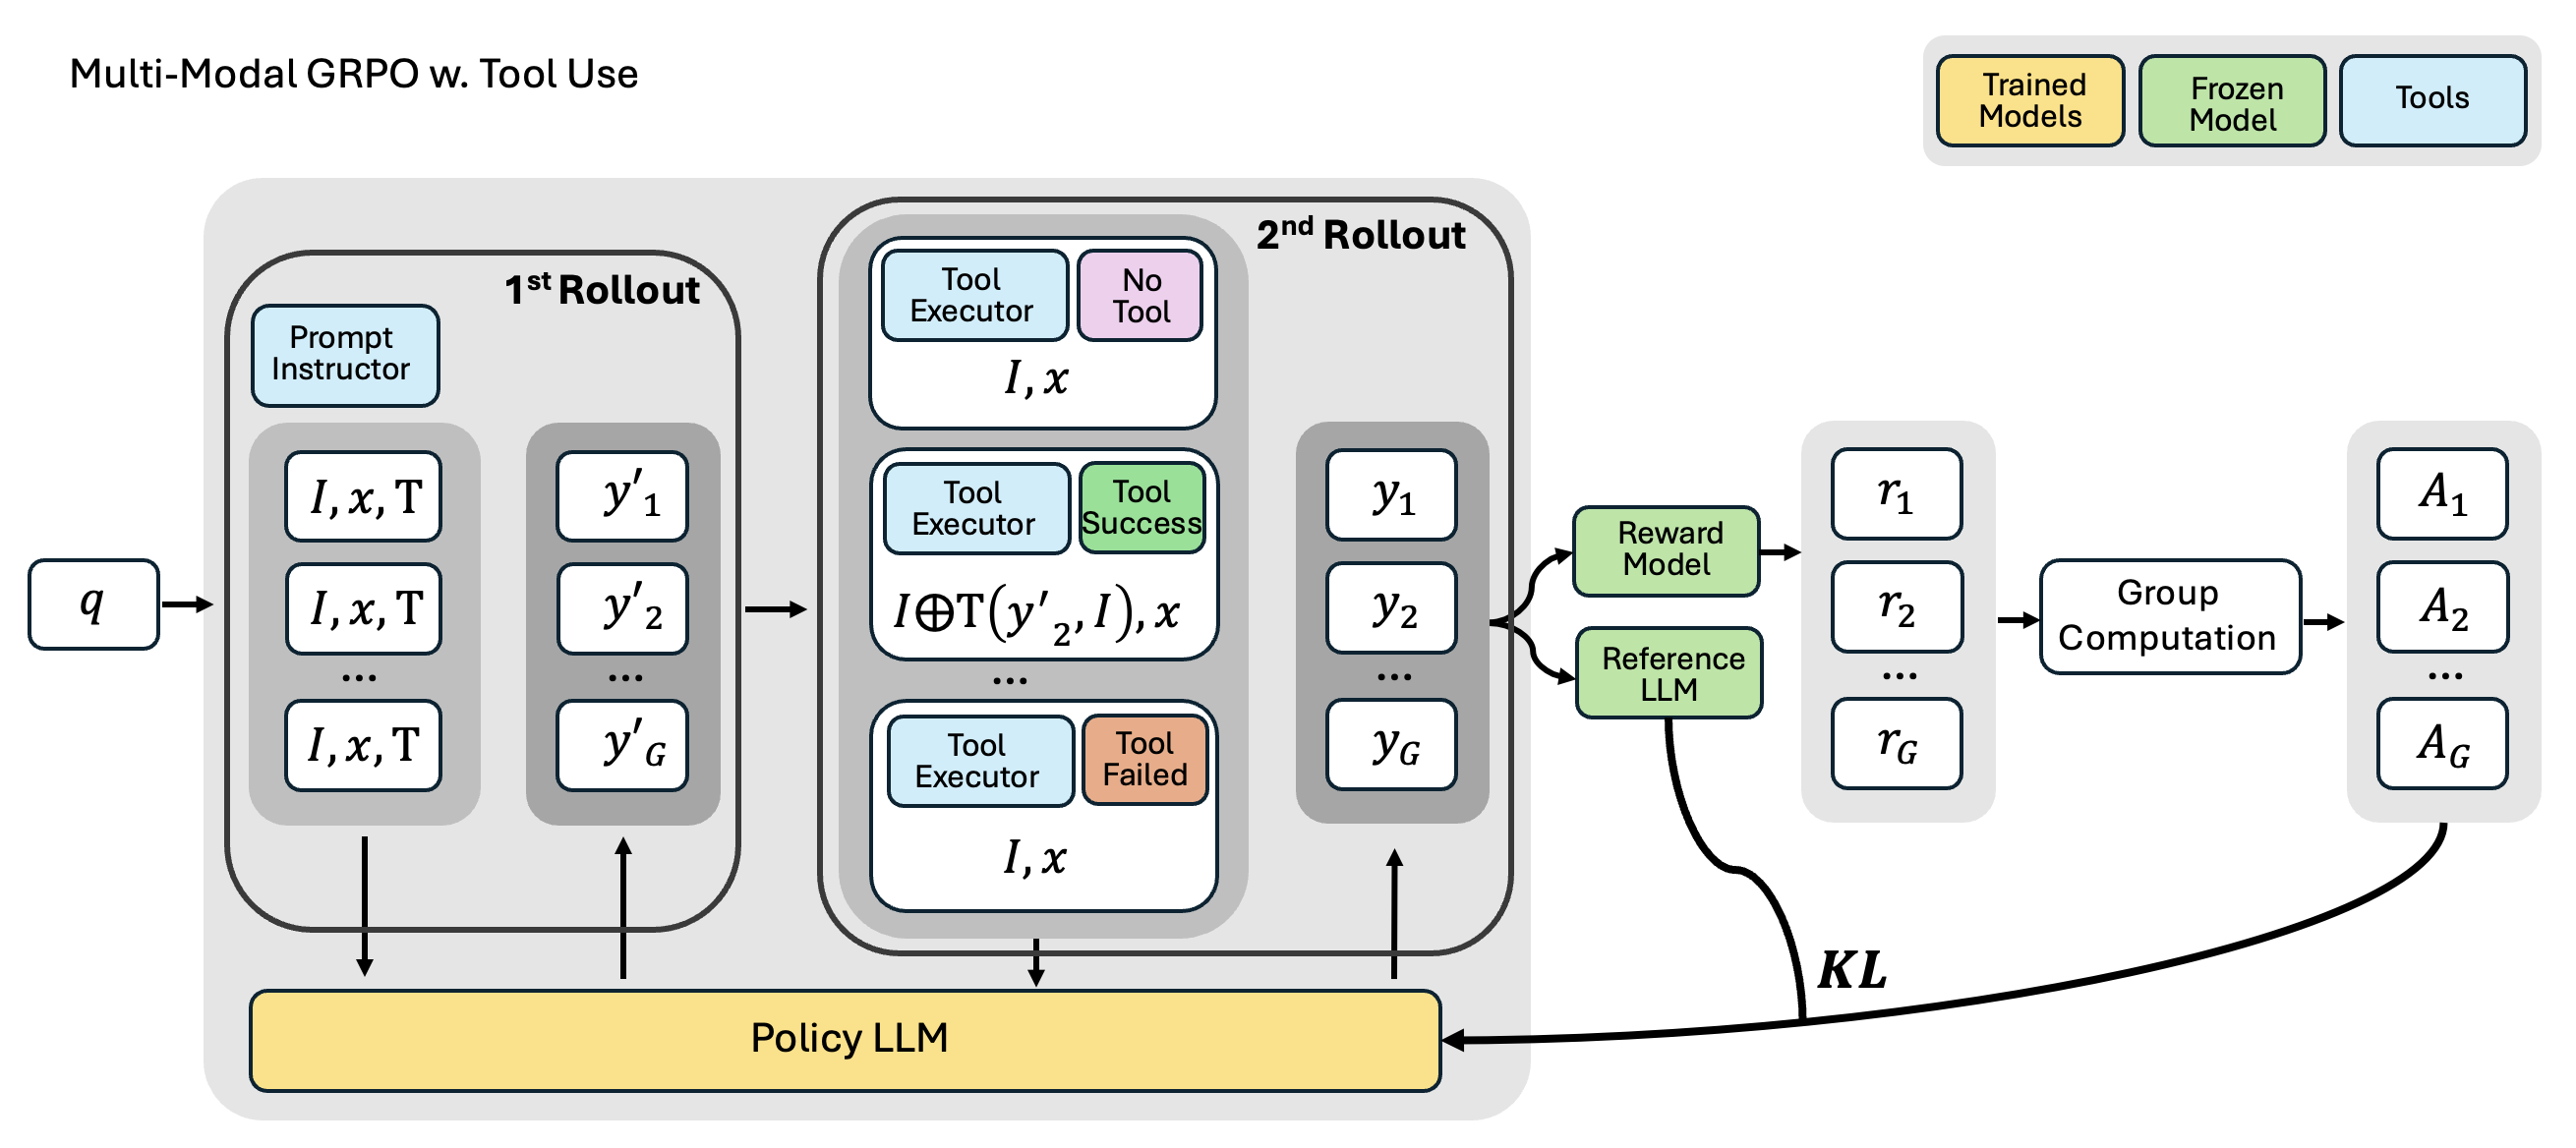
\includegraphics[width=0.8\textwidth]{tooluse_grpo.png}
    \caption{For each query $q$, $G$ first-pass responses $y'_i$ go through the tool executor: \emph{no tool}
      (answer from $I,x$), \emph{tool success} (2nd pass on $I\oplus\texttt{T}(y'_i,I)$), or \emph{tool failed}
      (fall back to $I,x$). Only the final $y_i$ are scored, turned into group-relative advantages $A_i$, and
      used to update the policy under a KL penalty to the frozen reference.}
  \end{figure}
\end{frame}

\begin{frame}{Core Design Choices and Why}
  \vspace{-0.2cm}
  \begin{columns}[T]
    \column{0.5\textwidth}
    \textbf{\textcolor{deepgold}{1. Optimize only the final response $y$}}
    \begin{itemize}\small
      \item The intermediate tool-call text $y'$ is not directly optimized.
      \item \emph{Why:} the goal is final answer quality; the model should decide on its own
            \emph{whether} a tool helps. More end-to-end.
    \end{itemize}
    \vspace{0.05cm}
    \textbf{\textcolor{deepgold}{2. Edited image fed back as a 2nd input}}
    \begin{itemize}\small
      \item Unlike Search-R1, the tool output is not spliced into the token sequence.
      \item \emph{Why:} the VLM must jointly attend to $I$ and $I'$; requires multi-image capability.
    \end{itemize}
    \column{0.5\textwidth}
    \textbf{\textcolor{deepgold}{3. Single tool turn}}
    \begin{itemize}\small
      \item One ACTION, possibly with several chained edits.
      \item \emph{Why:} multi-turn editing needs stronger multi-image VLMs; left as future work.
    \end{itemize}
    \vspace{0.05cm}
    \textbf{\textcolor{deepgold}{4. GRPO, no format reward}}
    \begin{itemize}\small
      \item Critic-free group baseline: cheaper and more stable than PPO for 16k-token,
            multi-image rollouts.
      \item Structured template + few-shot examples already give reliable formatting.
    \end{itemize}
  \end{columns}
  \vspace{0.1cm}
  \begin{block}{Central insight}
    \small Tools are only \emph{available} in the rollout and only correctness is rewarded,
    so tool use survives only where it actually helps.
  \end{block}
\end{frame}

\begin{frame}{Training Objective}
  \small
  \setlength{\abovedisplayskip}{4pt}\setlength{\belowdisplayskip}{4pt}
  \textbf{RL objective with tools in the rollout} (KL-regularized, Bradley--Terry reward $r_\phi$):
  $$ \max_{\pi_\theta}\;
     \mathbb{E}_{[I,x]\sim\mathcal{D},\; y\sim\pi_\theta(\cdot\mid I,x;\texttt{T})}\big[r_\phi(I,x,y)\big]
     \;-\;\beta\,\mathbb{D}_{\mathrm{KL}}\big[\pi_\theta(\cdot\mid I,x;\texttt{T})\,\|\,\pi_{\mathrm{ref}}(\cdot\mid I,x;\texttt{T})\big] $$
  \textbf{GRPO surrogate}, with a group $\{y_i\}_{i=1}^{G}\sim\pi_{\text{old}}(\cdot\mid I,x;\texttt{T})$:
  $$ \mathcal{J}_{\text{GRPO}}(\theta) = \mathbb{E}\Bigg[\frac{1}{G}\sum_{i=1}^{G}\frac{1}{|y_i|}\sum_{t=1}^{|y_i|}
     \min\!\Big(\rho_{i,t}(\theta)\hat{A}_{i,t},\;
     \mathrm{clip}\big(\rho_{i,t}(\theta),1-\epsilon,1+\epsilon\big)\hat{A}_{i,t}\Big)
     - \beta\,\mathbb{D}_{\mathrm{KL}}\big[\pi_\theta\,\|\,\pi_{\mathrm{ref}}\big]\Bigg] $$
  \vspace{-0.2cm}
  \begin{columns}[T]
    \column{0.5\textwidth}
    $$ \hat{A}_{i,t} = \frac{r_i - \mathrm{mean}(\mathbf{r})}{\mathrm{std}(\mathbf{r})} $$
    \column{0.48\textwidth}
    \footnotesize
    \begin{itemize}
      \item $\rho_{i,t}$: token-level probability ratio $\pi_\theta/\pi_{\text{old}}$ (written $r_{i,t}$ in the paper).
      \item $\hat{A}_{i,t}$: same advantage for every token of $y_i$, no critic.
      \item Only tokens of the final $y_i$ get gradient; $I'$ comes from the environment.
    \end{itemize}
  \end{columns}
\end{frame}

\begin{frame}{Reward Design: Outcome Only, and Why Process Rewards Fail}
  \small
  Reward: $r_i = 1$ if a lightweight \textbf{LLM judge} says the predicted answer matches the ground
  truth, else $0$ (``pseudo rule-based''; string match is too brittle for free-form chart/table answers).
  \vspace{0.3cm}
  \begin{columns}[T]
    \column{0.31\textwidth}
    \fcolorbox{medgreen}{white}{
      \parbox{0.92\textwidth}{\centering
        \textbf{\textcolor{medgreen}{Outcome reward (used)}}\\[0.1cm]
        \footnotesize 0/1 on final-answer correctness only.\\[0.1cm]
        Tool use rises and falls with its usefulness; accuracy improves steadily.
      }}
    \column{0.31\textwidth}
    \fcolorbox{alertred}{white}{
      \parbox{0.92\textwidth}{\centering
        \textbf{\textcolor{alertred}{Penalize failed tool calls}}\\[0.1cm]
        \footnotesize Model learns the safest policy:\\[0.1cm]
        \textbf{tool usage collapses to zero.}\\ ~
      }}
    \column{0.31\textwidth}
    \fcolorbox{alertred}{white}{
      \parbox{0.92\textwidth}{\centering
        \textbf{\textcolor{alertred}{Bonus for successful tool use}}\\[0.1cm]
        \footnotesize Model emits calls that merely \emph{trigger} the success check;\\[0.1cm]
        \textbf{hacking persists even with a stricter verifier.}
      }}
  \end{columns}
  \vspace{0.4cm}
  \begin{alertblock}{Takeaway}
    Rewarding the \emph{process} of tool use is easy to game. Rewarding only the \emph{outcome}
    is the most robust signal found by the authors (evidence is reported qualitatively, without a table).
  \end{alertblock}
\end{frame}

% =============================================================================
\section{Experiments \& Results}

\begin{frame}{Experimental Setup}
  \begin{columns}[T]
    \column{0.5\textwidth}
    \textbf{\textcolor{deepgold}{Data (exact ReFocus splits)}}
    \begin{itemize}\small
      \item \textbf{Table split:} VWTQ (750 QA, Wikipedia tables), VWTQ\_syn (250, synthetic styles),
            VTabFact (250, entailment). 70/30 train/test, no validation set.
      \item \textbf{Chart split:} ChartQA; 14,344 train / 813 val; test = 444 horizontal + 382 vertical bar charts.
    \end{itemize}
    \textbf{\textcolor{deepgold}{Models \& baselines}}
    \begin{itemize}\small
      \item Qwen2.5-VL 3B / 7B / 32B: \emph{Pure Run} (no tools) and \emph{Tool Use} (prompted, no RFT;
            regenerate on failed call).
      \item R1-VL 2B/7B (general visual RL), DeepEyes 7B (concurrent), GPT-4o (upper bound).
    \end{itemize}
    \column{0.47\textwidth}
    \textbf{\textcolor{deepgold}{Training (VeRL)}}
    \vspace{0.1cm}

    \resizebox{\textwidth}{!}{%
    \begin{tabular}{ll}
      \toprule
      Optimizer & AdamW, lr $10^{-6}$, wd $10^{-2}$ \\
      Max sequence & 16,384 tokens \\
      Global batch & 32 (table) / 256 (chart) \\
      Group size $G$ & 5 \\
      KL coeff.\ $\beta$ & $10^{-2}$ \\
      Decoding & temperature 1.0, bf16 \\
      Hardware & 3B/7B: 8/16$\times$H100; 32B: 8$\times$H200 \\
      \bottomrule
    \end{tabular}}
    \vspace{0.3cm}

    \small \textbf{Metric:} answer accuracy (\%) judged against ground truth.
  \end{columns}
\end{frame}

\begin{frame}{Main Results: Does RFT Teach Useful Tool Use?}
  \begin{center}
    \textbf{Accuracy (\%) of Qwen2.5-VL before and after VTool-R1}
    \vspace{0.15cm}

    \resizebox{0.82\textwidth}{!}{
      \begin{tabular}{lcccccc}
        \toprule
        \multirow{2}{*}{\textbf{Method}}
          & \multicolumn{2}{c}{\textbf{3B}} & \multicolumn{2}{c}{\textbf{7B}} & \multicolumn{2}{c}{\textbf{32B}} \\
        \cmidrule(lr){2-3} \cmidrule(lr){4-5} \cmidrule(lr){6-7}
        & \textbf{Chart} & \textbf{Table} & \textbf{Chart} & \textbf{Table} & \textbf{Chart} & \textbf{Table} \\
        \midrule
        Pure Run (no tools)     & \underline{51.8} & \underline{41.3} & \underline{76.2} & \underline{64.7} & \textbf{88.0} & \textbf{86.2} \\
        Tool Use (prompted)     & 24.6 & 24.3 & 53.4 & 41.1 & 85.0 & 76.0 \\
        \midrule
        \rowcolor{medgreen!10}
        \textbf{VTool-R1 (RFT)} & \textbf{64.0} & \textbf{57.9} & \textbf{80.7} & \textbf{71.7} & \underline{86.7} & \underline{84.5} \\
        \bottomrule
      \end{tabular}
    }
  \end{center}
  \vspace{0.2cm}
  \textbf{Key Takeaways:}
  \begin{itemize}\small
    \item \textcolor{medgreen}{\textbf{+12.2 / +16.6}} points over Pure Run at 3B (chart / table);
          \textcolor{medgreen}{\textbf{+4.5 / +7.0}} at 7B.
    \item Prompting small models to use tools \textcolor{alertred}{\textbf{costs 20--27 points}}; RFT turns the
          same tools from a liability into a gain (+39.4 / +33.6 at 3B).
    \item \textcolor{deepgold}{\textbf{At 32B the gain disappears:}} VTool-R1 recovers most of the tool-use drop
          but stays 1.3 / 1.7 points below Pure Run.
  \end{itemize}
\end{frame}

\begin{frame}{Comparison with Other RL-Tuned VLMs}
  \begin{center}
    \resizebox{0.72\textwidth}{!}{
      \begin{tabular}{llcc}
        \toprule
        \textbf{Model} & \textbf{Size} & \textbf{Chart} & \textbf{Table} \\
        \midrule
        R1-VL (general visual RL)  & 2B & 10.4 & 8.6 \\
        R1-VL (general visual RL)  & 7B & 63.8 & 45.4 \\
        DeepEyes (RL + zoom tools) & 7B & 60.0 & -- \\
        \midrule
        VTool-R1 & 3B & \underline{64.0} & \underline{57.9} \\
        \rowcolor{medgreen!10}
        \textbf{VTool-R1} & \textbf{7B} & \textbf{80.7} & \textbf{71.7} \\
        \midrule
        \textcolor{violet}{GPT-4o, Pure Run (upper bound)} & -- & \textcolor{violet}{82.9} & \textcolor{violet}{75.7} \\
        \textcolor{violet}{GPT-4o, Tool Use (ReFocus)}    & -- & \textcolor{violet}{80.5} & \textcolor{violet}{77.0} \\
        \bottomrule
      \end{tabular}
    }
  \end{center}
  \vspace{0.2cm}
  \begin{itemize}\small
    \item VTool-R1 3B already beats R1-VL 7B; the 7B model is within \textbf{2.2 / 4.0} points of GPT-4o.
    \item vs.\ concurrent DeepEyes: \textcolor{medgreen}{\textbf{80.7 vs.\ 60.0}} on charts, attributed to tools
          and tasks matched to structured images.
    \item \textcolor{alertred}{Caveat:} R1-VL and DeepEyes were not trained on these splits, so part of the gap
          is in-domain training, not tool use alone.
  \end{itemize}
\end{frame}

\begin{frame}{Training Dynamics: Tool Use Is Not Monotonic}
  \centering
  \begin{figure}
    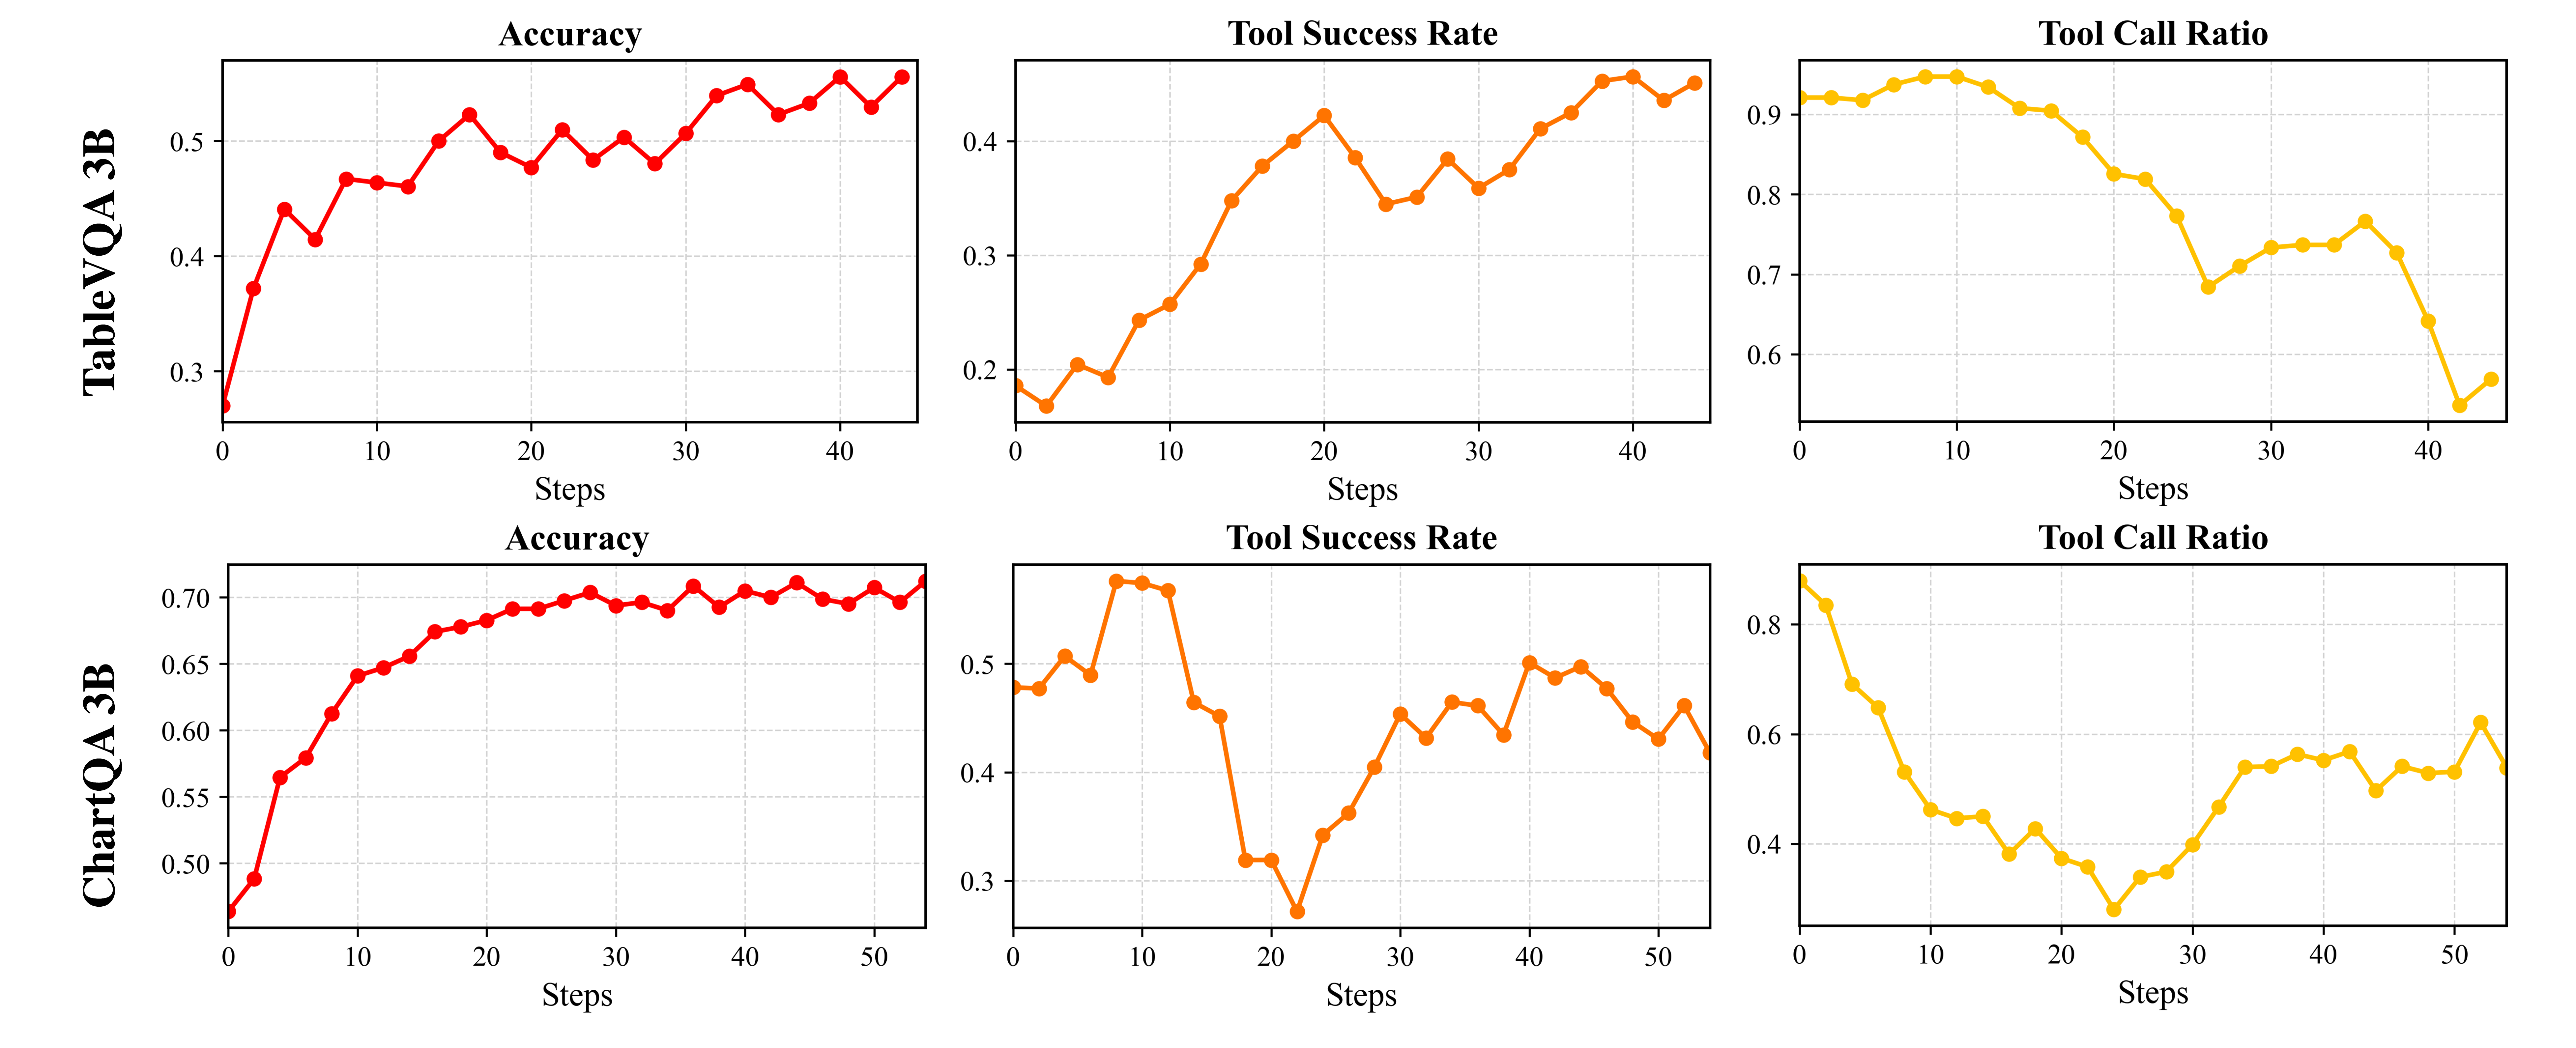
\includegraphics[width=0.74\textwidth]{new_vtool_fig1.png}
    \caption{3B training curves, TableVQA (top) and ChartQA (bottom). Accuracy rises
      (table $\approx$0.27$\rightarrow$0.55, chart $\approx$0.46$\rightarrow$0.71) and saturates in $\sim$50 steps,
      while the tool-call ratio \emph{falls} (table 0.92$\rightarrow$0.57; chart dips to 0.28, recovers to $\sim$0.55).}
  \end{figure}
  \vspace{-0.35cm}
  \begin{itemize}\footnotesize
    \item Prompt-driven over-use early on; later the model is \textbf{selective} and skips tools when unnecessary.
    \item Tool success (proxy: code runs, returns an image) climbs on tables, fluctuates on charts; 32B keeps a higher call ratio.
  \end{itemize}
\end{frame}

\begin{frame}{Failure Analysis}
  \vspace{-0.2cm}
  \begin{columns}[T]
    \column{0.38\textwidth}
    \centering
    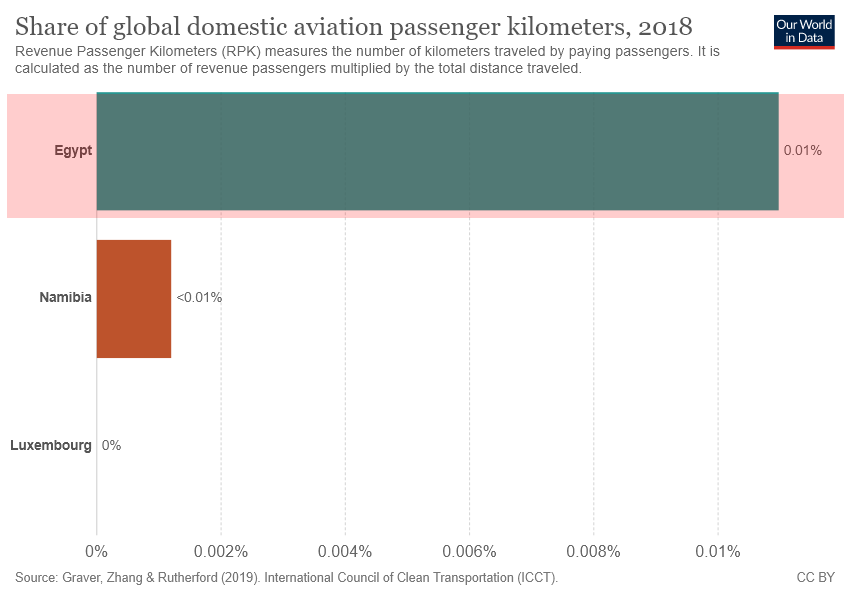
\includegraphics[width=\textwidth,trim=0 140 0 0,clip]{test-13001955010627_2_edited.png}\\[0.1cm]
    {\scriptsize\textbf{Case (a).} Q: ``What is the value of the largest bar?'' The tool correctly highlights Egypt
     and the 1st pass reads \textbf{0.01}, but the 2nd pass on the edited image says $\approx$0.001 and outputs
     ``Egypt''. GT: 0.01.}
    \column{0.6\textwidth}
    \textbf{\textcolor{alertred}{Four failure categories}}
    \begin{enumerate}\small
      \setlength{\itemsep}{0.05cm}
      \item[(a)] \textbf{Right visual step, wrong inference:} the 2nd rollout misreads or overrides a correct first-pass reading.
      \item[(b)] \textbf{Flawed edit:} the drawn box occludes the numbers it was meant to emphasize.
      \item[(c)] \textbf{Wrongly skips tools:} decides ``no action needed'' and answers incorrectly.
      \item[(d)] \textbf{Invalid code:} hallucinated APIs (e.g.\ \texttt{get\_children()}) fail, so no visual step is produced.
    \end{enumerate}
    \vspace{0.05cm}
    \begin{block}{Observation}
      \small Since $y'$ gets no gradient, a correct first-pass reading can be lost in the second pass;
      the visual step helps only if the 2nd pass actually uses it.
    \end{block}
  \end{columns}
\end{frame}

% =============================================================================
\section{Conclusion \& Future Work}

\begin{frame}{Current Limitations}
  \begin{columns}[T]
    \column{0.5\textwidth}
    \textbf{\textcolor{deepgold}{Stated by the authors}}
    \begin{itemize}
      \setlength{\itemsep}{0.3cm}
      \item \textbf{\textcolor{alertred}{Single tool turn only}}: no iterative edit--reason loops.
      \item \textbf{\textcolor{alertred}{Narrow scope}}: selective attention on charts and tables with a fixed toolset.
      \item \textbf{\textcolor{alertred}{No oracle for tool correctness}}: ``success'' only means the code ran.
    \end{itemize}
    \column{0.5\textwidth}
    \textbf{\textcolor{deepgold}{Our observations}}
    \begin{itemize}
      \setlength{\itemsep}{0.3cm}
      \item \textbf{\textcolor{alertred}{Tools need given bounding boxes}}: row/column/bar boxes are supplied in the prompt, which simplifies grounding.
      \item \textbf{\textcolor{alertred}{No benefit at 32B}}: gains shrink with scale; Pure Run wins at 32B.
      \item \textbf{\textcolor{alertred}{Missing ablation}}: no RFT run \emph{without} tools, so the gain from RL alone vs.\ RL + tools is not isolated.
      \item \textbf{\textcolor{alertred}{Reward-design evidence is qualitative}}; the LLM judge is itself a possible noise source.
    \end{itemize}
  \end{columns}
\end{frame}

\begin{frame}{Conclusion \& Takeaways}
  \begin{enumerate}
    \setlength{\itemsep}{0.45cm}
    \item \textbf{Framework:} VTool-R1 puts Python image-editing tools inside GRPO rollouts, so a VLM reasons over
          the original image $\oplus$ its own edited image.
    \item \textbf{Outcome-only reward is enough:} the model learns \emph{when} to use tools without process
          supervision, while process rewards get hacked.
    \item \textbf{Results:} 3B/7B Qwen2.5-VL gain up to \textcolor{medgreen}{\textbf{+16.6}} points over direct
          answering; 7B approaches GPT-4o on chart and table QA.
    \item \textbf{Outlook:} multi-turn editing, richer (generative) tools, and broader tasks beyond structured images.
  \end{enumerate}
  \vspace{0.5cm}
  \begin{center}
    \large \textbf{Thank You!}\\[0.1cm]
    \normalsize Questions?
  \end{center}
\end{frame}

% =============================================================================
\section{References}
\begin{frame}[allowframebreaks]{References}
  \scriptsize
  \begin{thebibliography}{99}
  \bibitem{vtool} Wu, M., Yang, J., Jiang, J., et al. (2025). VTool-R1: VLMs Learn to Think with Images via Reinforcement Learning on Multimodal Tool Use. \emph{arXiv:2505.19255}.
  \bibitem{refocus} Fu, X., Liu, M., Yang, Z., et al. (2025). ReFocus: Visual Editing as a Chain of Thought for Structured Image Understanding. \emph{ICML}.
  \bibitem{sketchpad} Hu, Y., Shi, W., Fu, X., et al. (2024). Visual Sketchpad: Sketching as a Visual Chain of Thought for Multimodal Language Models. \emph{NeurIPS}.
  \bibitem{r1} DeepSeek-AI. (2025). DeepSeek-R1: Incentivizing Reasoning Capability in LLMs via Reinforcement Learning. \emph{arXiv:2501.12948}.
  \bibitem{grpo} Shao, Z., Wang, P., Zhu, Q., et al. (2024). DeepSeekMath: Pushing the Limits of Mathematical Reasoning in Open Language Models. \emph{arXiv:2402.03300}.
  \bibitem{ppo} Schulman, J., Wolski, F., Dhariwal, P., et al. (2017). Proximal Policy Optimization Algorithms. \emph{arXiv:1707.06347}.
  \bibitem{searchr1} Jin, B., Zeng, H., Yue, Z., et al. (2025). Search-R1: Training LLMs to Reason and Leverage Search Engines with Reinforcement Learning. \emph{arXiv:2503.09516}.
  \bibitem{qwen} Bai, S., Chen, K., Liu, X., et al. (2025). Qwen2.5-VL Technical Report. \emph{arXiv:2502.13923}.
  \bibitem{r1vl} Zhang, J., Huang, J., Yao, H., et al. (2025). R1-VL: Learning to Reason with Multimodal Large Language Models via Step-wise Group Relative Policy Optimization. \emph{arXiv:2503.12937}.
  \bibitem{deepeyes} Zheng, Z., Yang, M., Hong, J., et al. (2025). DeepEyes: Incentivizing ``Thinking with Images'' via Reinforcement Learning. \emph{arXiv:2505.14362}.
  \bibitem{verl} Sheng, G., Zhang, C., Ye, Z., et al. (2024). HybridFlow: A Flexible and Efficient RLHF Framework. \emph{arXiv:2409.19256}.
  \bibitem{chartqa} Masry, A., Long, D.~X., Tan, J.~Q., et al. (2022). ChartQA: A Benchmark for Question Answering about Charts with Visual and Logical Reasoning. \emph{Findings of ACL}.
  \bibitem{tablevqa} Kim, Y., Yim, M., \& Song, K.~Y. (2024). TableVQA-Bench: A Visual Question Answering Benchmark on Multiple Table Domains. \emph{arXiv:2404.19205}.
  \bibitem{wtq} Pasupat, P., \& Liang, P. (2015). Compositional Semantic Parsing on Semi-Structured Tables. \emph{ACL}.
  \bibitem{tabfact} Chen, W., Wang, H., Chen, J., et al. (2020). TabFact: A Large-scale Dataset for Table-based Fact Verification. \emph{ICLR}.
  \end{thebibliography}
\end{frame}

\end{document}
